% ============================================================
% Capstone Project Proposal
% Improving Grasp Planning for Mobile Manipulators through
% Coordinated Base-Arm Motion Control
%
% Overleaf-ready. Compile with pdfLaTeX.
% Title page intentionally omitted.
% ============================================================

\documentclass[12pt,a4paper]{article}

\usepackage[T1]{fontenc}
\usepackage[utf8]{inputenc}
\usepackage{lmodern}
\usepackage[margin=1in]{geometry}
\usepackage{amsmath,amssymb}
\usepackage{graphicx}
\usepackage{subcaption}
\usepackage{setspace}
\usepackage{enumitem}
\usepackage{titlesec}
\usepackage[hidelinks]{hyperref}
\usepackage{xcolor}
\graphicspath{{figures/}{images/}}

\bibliographystyle{plain} % or apalike for APA-like style
  

\onehalfspacing
\setlength{\parindent}{0.5in}
\setlist[itemize]{itemsep=2pt,topsep=4pt}
\setlist[enumerate]{itemsep=2pt,topsep=4pt}

\titleformat{\section}{\normalfont\large\bfseries}{\thesection}{1em}{}
\titleformat{\subsection}{\normalfont\normalsize\bfseries}{\thesubsection}{1em}{}
\titleformat{\subsubsection}{\normalfont\normalsize\itshape}{\thesubsubsection}{1em}{}

% --- Placeholder box for figures that are not yet inserted -------------
% Replace \figplaceholder{...}{...} with \includegraphics when the real
% image files are available.
% \begin{figure}
%     \centering
%     
\includegraphics[width=0.5\linewidth]{chula_logo_thumb.png}
% \end{figure}
\newcommand{\figplaceholder}[2]{%
  \fbox{\begin{minipage}[c][#2][c]{#1}
    \centering \textit{[ Image placeholder ]}
  \end{minipage}}%
}

\begin{document}

% ============================================================
% TITLE PAGE
% ============================================================
\begin{titlepage}
\centering
\thispagestyle{empty}
\vspace*{0.8in}

% ---------------- LOGO PLACEHOLDER --------------------------
% Replace the placeholder below with:
%   \includegraphics[width=0.40\textwidth]{chula_logo.png}
% \figplaceholder{0.40\textwidth}{3cm}
% \begin{figure}
%     \centering
%     
\includegraphics[width=0.5\linewidth]{chula_logo_thumb.png}
% \end{figure}

\includegraphics[width=0.40\textwidth]{chula_logo.jpg}
% ------------------------------------------------------------

\vspace{0.5in}

{\LARGE\bfseries Capstone Project First Progress Report\par}

\vspace{0.35in}

{\large\bfseries Topic\par}
\vspace{0.10in}
{\large Improving Grasp Planning for Mobile Manipulators through\\
Coordinated Base--Arm Motion Control\par}

\vspace{0.55in}

{\large\bfseries Advisor\par}
\vspace{0.10in}
{\large Assoc.Prof. Ronnapee Chaichaowarat, Ph.D.\par}

\vspace{0.55in}

{\large\bfseries Submitted By\par}
\vspace{0.10in}
{\large
Supphakorn Akkapoo 6638226721\\
Natapol Chusang 6638050521\\
Taratorn Assawadejmetakul 6638087821\par}

\vspace{0.55in}

{\large\bfseries Majors\par}
\vspace{0.10in}
{\large Robotics and Artificial Intelligence Engineering\par}

\vfill
\end{titlepage}

\setcounter{page}{1}

% ============================================================
\section*{Traditional Control Approach}

For the traditional model-based approach, the project repository has been established on \textcolor{blue}{\href{https://github.com/MonochromePie/Coordinated-Base-Arm-Motion-Control}{GitHub}} and the initial simulation environment has been implemented.

Instead of using Gazebo or Isaac Sim, MuJoCo was selected for the initial simulation because it provides a simpler environment for developing and testing the planned kinematic and control methods. The control methods investigated in this stage are primarily focused on the robot's kinematic configuration and joint-level motion, making MuJoCo suitable for rapid development and experimentation at the current stage.

Since a complete simulation model of the Walkie mobile base is not yet available, an existing OpenArm XML model was used as the starting point. The model was modified to introduce additional virtual joints representing the mobile base's degrees of freedom, namely $X$, $Y$, $Z$, and yaw. This allows the mobile base and manipulator to be represented within a single kinematic chain and provides an initial environment for developing the proposed coordinated base--arm motion planning approach.

\begin{center}
    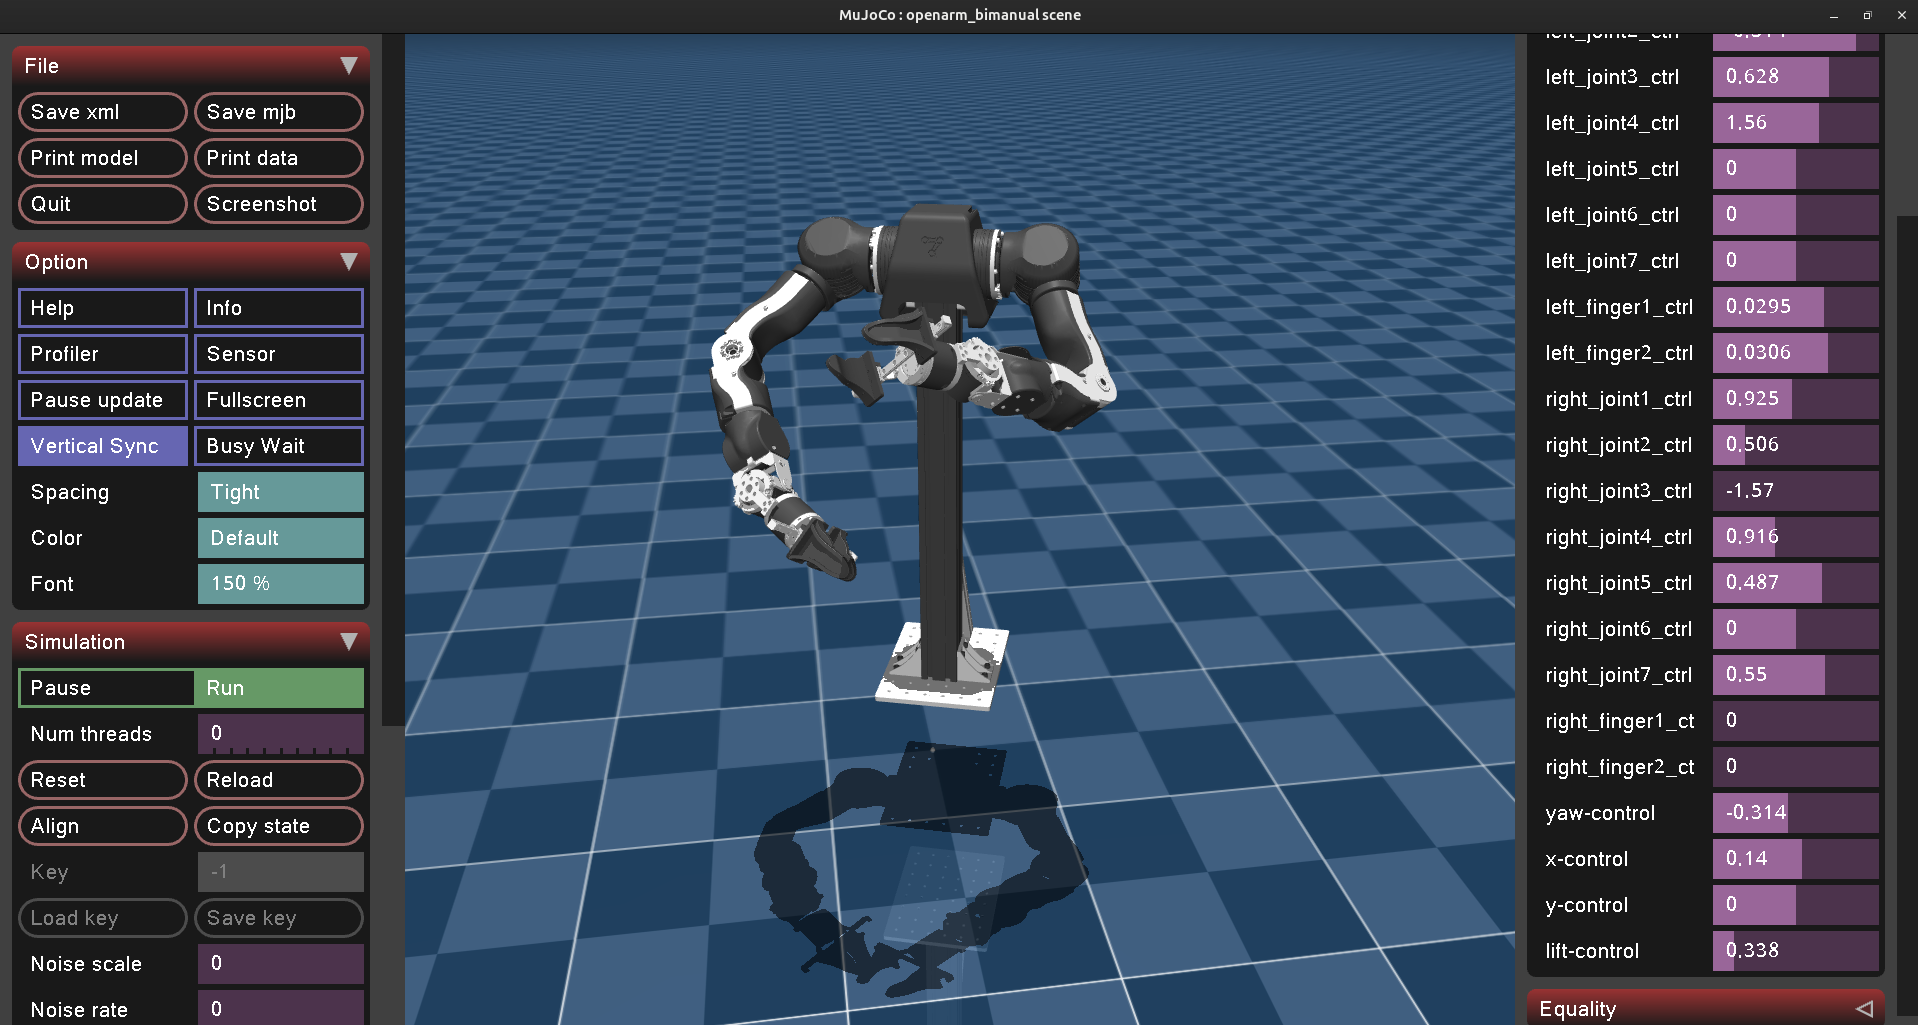
\includegraphics[scale=0.15]{Mujoco_walker.png}\\
    \textit{\small{MuJoCo simulation of the unified mobile base--arm model with control interface.}}
\end{center}

The current simulation demonstrates the combined configuration of the virtual mobile base and OpenArm manipulator. This serves as a preliminary validation of the unified model before integrating the approach with the actual Walkie simulation once its simulation model becomes available. A \textcolor{blue}{\href{https://youtu.be/VUVee6bROx8}{demonstration video}} of the current MuJoCo simulation is also available as part of the progress report.

Following the initial unified-model implementation, the simulation work is being developed along two parallel directions. The first direction focuses on integrating the unified mobile base--arm model into MoveIt to evaluate its kinematic behaviour using an established robotics framework. The wheel base and manipulator are being combined into a single model to investigate whether the proposed coordinated base--arm control method can be implemented within the MoveIt framework and to evaluate its behaviour using the available kinematic and planning tools.

The second direction continues development within MuJoCo by implementing the required control components independently. This includes developing the inverse kinematics, motion control, and path planning methods directly within the simulation environment. This approach provides greater control over the implementation and allows the proposed method to be tested independently of existing planning frameworks.

These two approaches will be used in parallel to evaluate the feasibility of the proposed coordinated base--arm motion planning method. The MoveIt implementation provides an opportunity to validate the approach using an established robotics framework, while the custom MuJoCo implementation allows the underlying kinematics, control, and planning methods to be developed and evaluated directly.


\section*{VLA Control Approach}
    To establish an implementation baseline, a preliminary simulation is set up to reproduce experimental results. $\pi$ 0.5 \cite{intelligence2025pi05visionlanguageactionmodelopenworld} 
    is chosen as a preliminary model due to its abundance of community resources and widespread support across many software. NVIDIA's Issac sim is used as the simulation software to mimic experimental results.Le-robot's lehome\cite{li2026lehomesimulationenvironmentdeformable} is used as the simulation environment due to its ease of use and support for standard benchmark tasks. As the original $\pi$ 0.5 paper did not provide its training data or methodology, Open-source datasets and training parameters are being considered for training. Preliminary training progress and benchmarks will likely be availabe on the next progress report.

    \begin{center}
    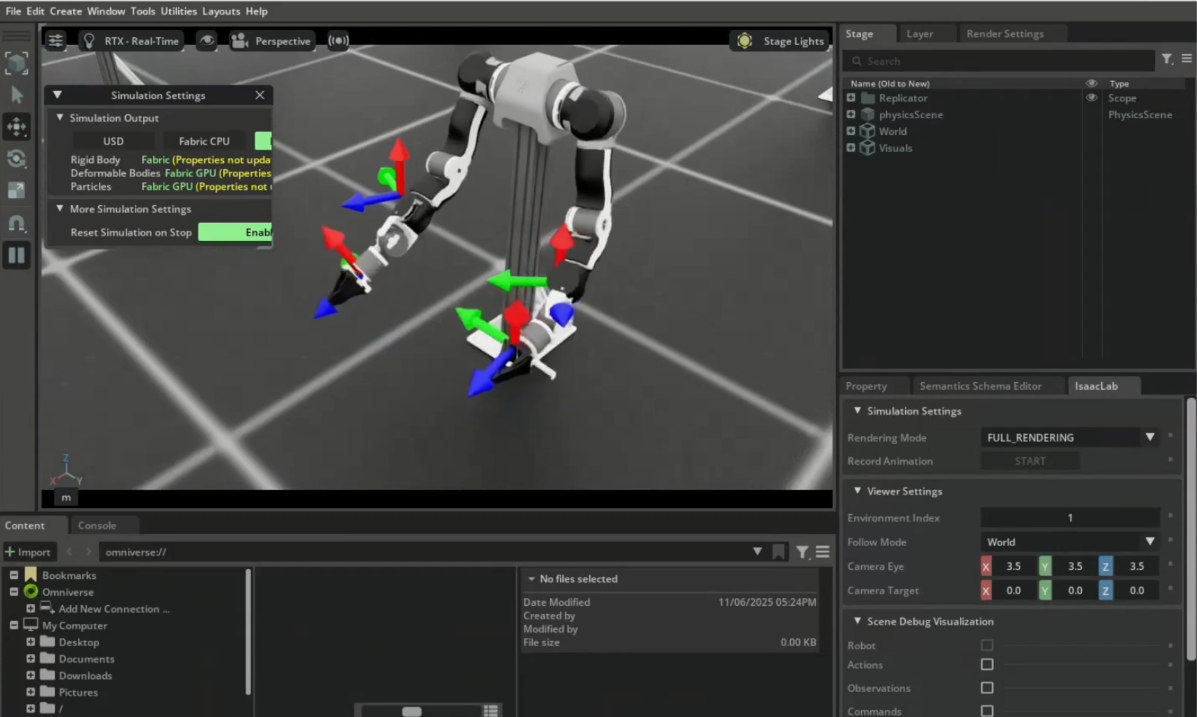
\includegraphics[scale=0.75]{openarmissac.png}\\
    \textit{\small{IssacSim of OpenArm}}
\end{center}

\bibliography{citations} 

\end{document}